\chapter{缓冲溶液与优势区域图}\label{ch:g12:buffers-predominance}

血液检验报告动脉血的 pH：正常时介于 7.38 与
7.42 之间。运动中的肌肉向血液中释放酸，肺将
二氧化碳排出血液，食物带入酸和碱；然而 pH
几乎不变。一个酸碱共轭对，即一种酸及其自身的共轭碱，能吸收这些冲击。
本章说明：在给定 pH 下，哪种形式的共轭对占优势，
几滴有色共轭对如何显示 pH，
以及酸与其共轭碱的混合物如何使 pH 保持稳定。

\begin{recall}
酸碱共轭对、$K_a$ 与 $pK_a$；溶液的 pH
（见\cref{ch:g12:ka-and-pka}，\cref{ch:g9:acids-bases-ph}）。
\end{recall}

\begin{omfigure}
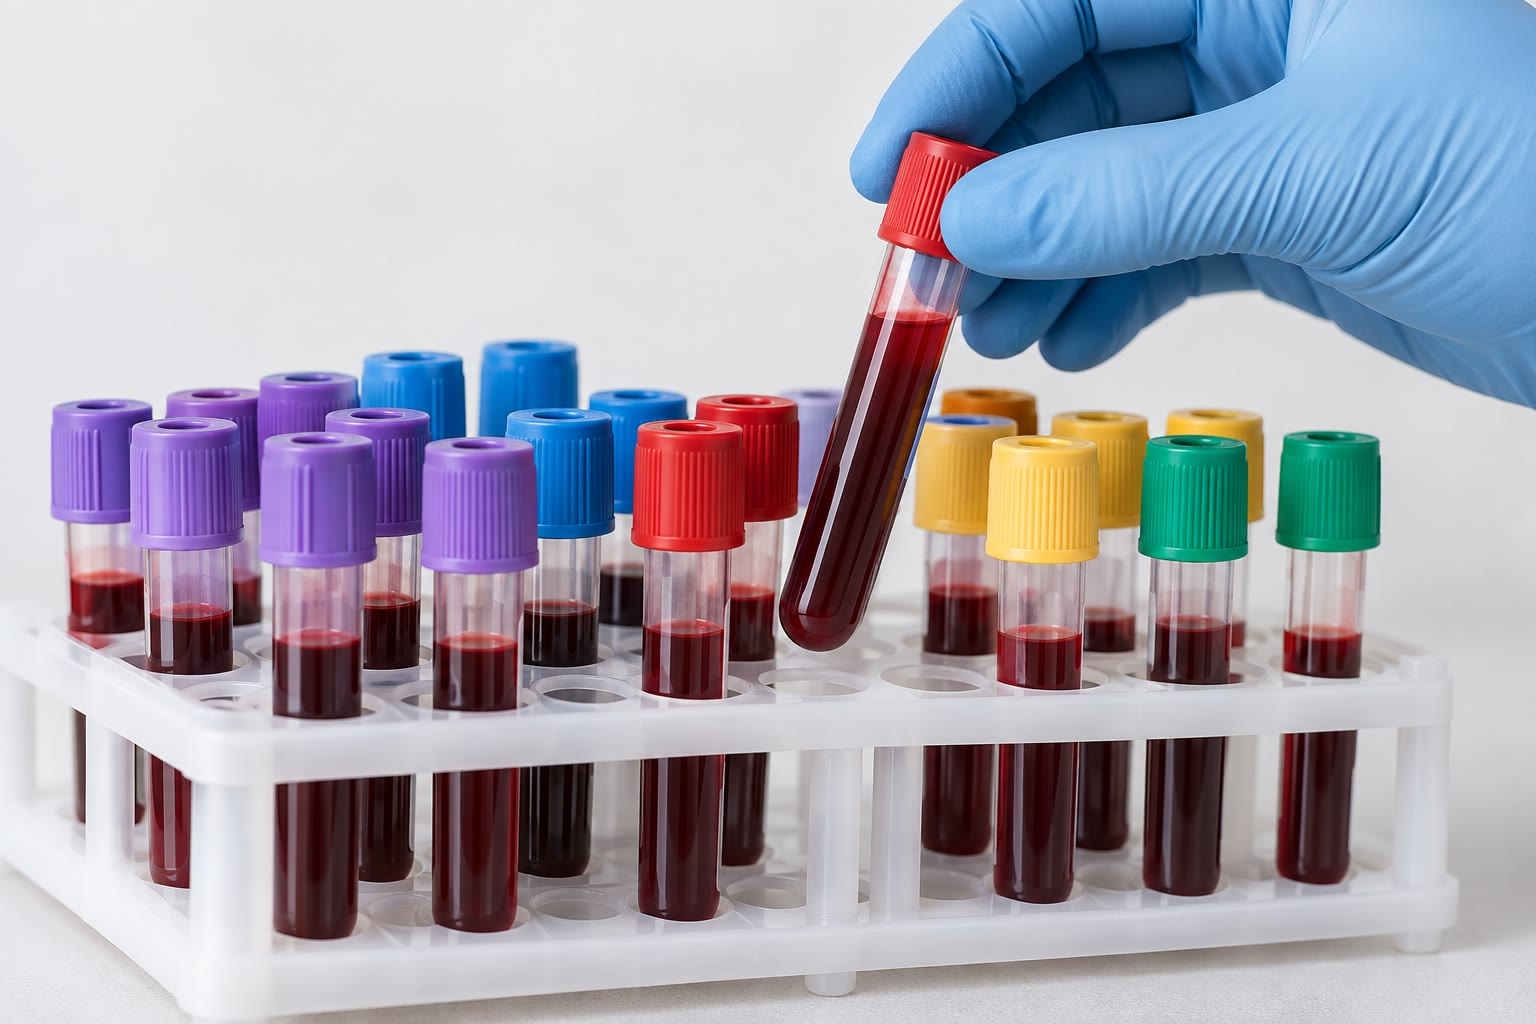
\includegraphics[width=0.45\linewidth]{images/book1/ai/g12-blood-tubes.jpg}

{\small 血样：其 pH 维持在很窄的范围内。}
\end{omfigure}

\section{优势区域图}

\begin{proposition}[亨德森关系式]\label{prop:g12:buffers-predominance:henderson}
在含有共轭对 \ce{HA}/\ce{A-} 的任意水溶液中，
\[
  \mathrm{pH} = pK_a + \log\frac{[\ce{A-}]}{[\ce{HA}]} .
\]
\end{proposition}

\begin{proof}
由 $K_a = \dfrac{[\ce{A-}][\ce{H3O+}]}{[\ce{HA}]c^\circ}$，两边取 $-\log$
得 $pK_a = \mathrm{pH} - \log\dfrac{[\ce{A-}]}{[\ce{HA}]}$。
\end{proof}

\begin{definition}[优势区域图与分布图]\label{def:g12:buffers-predominance:predominance}
共轭对的\emph{优势区域图}\index{优势区域图}是在
$pK_a$ 处分割的 pH 轴：低于此值时，酸 HA 占优势
（$[\ce{HA}] > [\ce{A-}]$），在其上方则碱 \ce{A-} 占优势。\emph{分布
图}\index{分布图}给出每种形式所占的分数，
即 $[\ce{HA}]/c$ 与 $[\ce{A-}]/c$ 随 pH 的变化；两条曲线在
$\mathrm{pH} = pK_a$ 处相交。
\end{definition}

\begin{method}[绘制优势区域图]\label{met:g12:buffers-predominance:diagram}
\begin{enumerate}
  \item 画一条从 0 到 14 的 pH 轴，并标出共轭对的 $pK_a$。
  \item 在 $pK_a$ 左侧写出酸，右侧写出碱。
  \item 对于有多个共轭对的物种（如可给出两个质子的酸、氨基酸），
        标出所有 $pK_a$：每个区间
        只属于一种形式。
  \item 距 $pK_a$ 一个 pH 单位时，两种形式之比已为 10 比 1：次要
        形式的含量低于 \qty{10}{\percent}。
\end{enumerate}
\end{method}

\begin{omfigure}
\begin{tikzpicture}[font=\small, x=0.62cm]
  % ledger: pka:ethanoic, pka:methanoic, kb:NH3, ka:H2CO3
  \foreach \y/\pk/\acid/\base in {0/3.74/{\ce{HCOOH}}/{\ce{HCOO-}},
      -1.0/4.76/{\ce{CH3COOH}}/{\ce{CH3COO-}}, -2.0/6.37/{\ce{CO2,H2O}}/{\ce{HCO3-}},
      -3.0/9.26/{\ce{NH4+}}/{\ce{NH3}}} {
    \fill[omThm!20] (0,\y) rectangle (\pk,\y+0.5);
    \fill[omDef!20] (\pk,\y) rectangle (14,\y+0.5);
    \draw[black!50] (0,\y) rectangle (14,\y+0.5);
    \node at (\pk/2,\y+0.25) {\acid};
    \node at ({(\pk+14)/2},\y+0.25) {\base};
    \draw[thick] (\pk,\y-0.08) -- (\pk,\y+0.58);
    \node[font=\scriptsize, anchor=south] at (\pk,\y+0.55) {\pk};
  }
  \draw[->] (0,-3.4) -- (14.5,-3.4) node[right] {pH};
  \foreach \k in {0,2,4,6,8,10,12,14} \draw (\k,-3.35) -- (\k,-3.45) node[below, font=\scriptsize] {\k};
\end{tikzpicture}

{\small 四组共轭对的优势区域图：酸（左侧，红色）
在 $pK_a$ 以下占优势，碱（右侧，蓝色）在其上方占优势。}
\end{omfigure}

\begin{omfigure}
\begin{minipage}{0.49\linewidth}
\begin{tikzpicture}
\begin{axis}[width=\linewidth, height=5cm, xmin=0, xmax=14, ymin=0, ymax=1.05,
    xlabel={pH}, ylabel={分数}, axis lines*=left, ymajorgrids,
    grid style={gray!20}, tick label style={font=\scriptsize},
    label style={font=\small}, title={\small 乙酸},
    title style={yshift=-4pt}]
  \addplot[very thick, omThm] table[x=pH, y=HA] {figdata/out/grade-12-buffers-predominance-a.dat};
  \addplot[very thick, omDef] table[x=pH, y=A] {figdata/out/grade-12-buffers-predominance-a.dat};
  \addplot[dashed, black!50] coordinates {(4.76,0) (4.76,1)};
  \node[font=\scriptsize, omThm] at (axis cs:2.2,0.85) {\ce{CH3COOH}};
  \node[font=\scriptsize, omDef] at (axis cs:7.6,0.85) {\ce{CH3COO-}};
\end{axis}
\end{tikzpicture}
\end{minipage}\hfill
\begin{minipage}{0.49\linewidth}
\begin{tikzpicture}
\begin{axis}[width=\linewidth, height=5cm, xmin=0, xmax=14, ymin=0, ymax=1.05,
    xlabel={pH}, ylabel={分数}, axis lines*=left, ymajorgrids,
    grid style={gray!20}, tick label style={font=\scriptsize},
    label style={font=\small}, title={\small 甘氨酸},
    title style={yshift=-4pt}]
  \addplot[very thick, omThm] table[x=pH, y=cation] {figdata/out/grade-12-buffers-predominance-b.dat};
  \addplot[very thick, omMeth] table[x=pH, y=zwitterion] {figdata/out/grade-12-buffers-predominance-b.dat};
  \addplot[very thick, omDef] table[x=pH, y=anion] {figdata/out/grade-12-buffers-predominance-b.dat};
  \node[font=\scriptsize, omThm] at (axis cs:1.0,0.55) {阳离子};
  \node[font=\scriptsize, omMeth] at (axis cs:6.1,0.88) {两性离子};
  \node[font=\scriptsize, omDef] at (axis cs:12.6,0.55) {阴离子};
\end{axis}
\end{tikzpicture}
\end{minipage}

{\small 由 $pK_a$ 值算得的分布图。左：
乙酸，两曲线在 4.76 处相交。右：甘氨酸，
\ce{H2N-CH2-COOH}，有两个共轭对（$pK_a$ 为 2.35 和 9.78）：阳离子
\ce{H3N+-CH2-COOH}、两性离子 \ce{H3N+-CH2-COO-} 和阴离子
\ce{H2N-CH2-COO-}。}
\end{omfigure}

\begin{example}[甘氨酸在人体内]\label{ex:g12:buffers-predominance:glycine}
% ledger: pka:glycine1, pka:glycine2, ph:blood
血液的 pH 约为 7.4，此时甘氨酸处于其两个 $pK_a$
值之间：它几乎全部以两性离子形式存在，带
正电荷的是氮原子，带负电荷的是羧酸根，
整体呈电中性。每种氨基酸都是如此。
\end{example}

\section{酸碱指示剂}


\begin{definition}[酸碱指示剂、变色范围]\label{def:g12:buffers-predominance:indicator}
\emph{酸碱指示剂}\index{酸碱指示剂}是一个酸碱共轭对
\ce{HInd}/\ce{Ind-}，其两种形式颜色不同，用量很少。
其\emph{变色范围}\index{变色范围}
为颜色可见发生变化的 pH 区间，大致为
$pK_a - 1$ 至 $pK_a + 1$：pH 低于此值时看到 \ce{HInd} 的颜色，高于此值时
看到 \ce{Ind-} 的颜色，两者之间则为二者的混合色。
\end{definition}

\begin{omfigure}
\begin{tikzpicture}[font=\small, x=0.62cm]
  % ledger: ind:methyl-red, ind:BBT, ind:phenolphthalein, ind:thymol-blue, ind:range-rule
  \foreach \y/\name/\a/\b/\ca/\cm/\cb in {
      0/{methyl red}/4.2/6.3/red!70/orange/yellow!80,
      -0.8/{bromothymol blue}/6.0/7.6/yellow!80/green!60/blue!60,
      -1.6/{phenolphthalein}/8.0/10.0/white/magenta!25/magenta!70} {
    \fill[\ca] (0,\y) rectangle (\a,\y+0.5);
    \shade[left color=\ca, right color=\cb] (\a,\y) rectangle (\b,\y+0.5);
    \fill[\cb] (\b,\y) rectangle (14,\y+0.5);
    \draw[black!50] (0,\y) rectangle (14,\y+0.5);
    \node[anchor=east] at (-0.2,\y+0.25) {\name};
  }
  \fill[red!65] (0,-2.4) rectangle (1.2,-1.9);
  \shade[left color=red!65, right color=yellow!80] (1.2,-2.4) rectangle (2.8,-1.9);
  \fill[yellow!80] (2.8,-2.4) rectangle (8.0,-1.9);
  \shade[left color=yellow!80, right color=blue!60] (8.0,-2.4) rectangle (9.1,-1.9);
  \fill[blue!60] (9.1,-2.4) rectangle (14,-1.9);
  \draw[black!50] (0,-2.4) rectangle (14,-1.9);
  \node[anchor=east] at (-0.2,-2.15) {百里酚蓝};
  \draw[->] (0,-2.8) -- (14.5,-2.8) node[right] {pH};
  \foreach \k in {0,2,4,6,8,10,12,14} \draw (\k,-2.75) -- (\k,-2.85) node[below, font=\scriptsize] {\k};
\end{tikzpicture}

{\small 四种指示剂的颜色随 pH 变化的情况如图，阴影部分为
变色范围。百里酚蓝含两个共轭对，因此有两个
变色范围。}
\end{omfigure}

\begin{method}[选择指示剂]\label{met:g12:buffers-predominance:indicator}
要检测溶液何时到达某一给定 pH（例如滴定的终点 pH），
应选择变色范围包含该 pH 的指示剂，
此时颜色恰好在该处发生变化。
\end{method}

\section{缓冲溶液}

\begin{definition}[缓冲溶液]\label{def:g12:buffers-predominance:buffer}
\emph{缓冲溶液}\index{缓冲溶液}是一种溶液，其 pH
在加入少量酸或碱时，或被稀释时变化很小。
通常由弱酸及其共轭碱按
相近的量配制，此时其 pH 接近该共轭对的 $pK_a$。
\end{definition}

\begin{proposition}[缓冲溶液为何能抵抗变化]\label{prop:g12:buffers-predominance:buffer}
在由 \ce{HA} 和 \ce{A-} 组成的缓冲溶液中，加入的强酸被 \ce{A-}
消耗（\ce{A- + H3O+ -> HA + H2O}），加入的强碱则被 \ce{HA}
消耗（\ce{HA + OH- -> A- + H2O}）；比值 $[\ce{A-}]/[\ce{HA}]$ 因而
pH 只发生很小的变化。稀释根本不改变该比值。
\end{proposition}

\begin{proof}
由亨德森方程可知，pH 仅取决于该比值。向
两种形式各含 \qty{10}{mmol} 的缓冲溶液中加入 \qty{1}{mmol} 酸，
比值由 $10/10$ 变为 $9/11$，pH 的变化量
仅为 $\log(9/11) = -0.09$。
\end{proof}

\begin{omfigure}
\begin{tikzpicture}
\begin{axis}[width=0.75\linewidth, height=5.6cm, xmin=0, xmax=10, ymin=0,
    ymax=8, xlabel={加入 \ce{HCl}（\qty{0.10}{mol/L}）的体积（\si{mL}）},
    ylabel={pH}, axis lines*=left, ymajorgrids, grid style={gray!20},
    tick label style={font=\small}, label style={font=\small},
    legend style={font=\small, at={(0.98,0.97)}, anchor=north east,
    draw=none, fill=white}, legend cell align=left]
  % ledger: pka:ethanoic (buffer recipe: exercise data)
  \addplot[very thick, omThm, mark=*, mark size=1.3pt] table[x=V, y=water]
    {figdata/out/grade-12-buffers-predominance-c.dat};
  \addplot[very thick, omDef, mark=*, mark size=1.3pt] table[x=V, y=buffer]
    {figdata/out/grade-12-buffers-predominance-c.dat};
  \legend{\qty{100}{mL} 纯水，\qty{100}{mL} 乙酸盐缓冲溶液}
\end{axis}
\end{tikzpicture}

{\small 向纯水及由乙酸和乙酸钠组成的缓冲溶液中分别加入盐酸，
（各 \qty{0.10}{mol/L}）。纯水的 pH
由 7 降至约 2，缓冲溶液的 pH 则由 4.76 降至 4.67。}
\end{omfigure}

\begin{method}[配制缓冲溶液]\label{met:g12:buffers-predominance:prepare}
\begin{enumerate}
  \item 选择一个 $pK_a$ 与所需 pH 相差不超过一个单位的共轭对，
        （最好尽量接近）。
  \item 计算比值 $[\ce{A-}]/[\ce{HA}] = 10^{\mathrm{pH} - pK_a}$。
  \item 按该比值将弱酸与其碱的盐混合，
        浓度要足够高，使所加入的
        酸或碱能被吸收。
\end{enumerate}
\end{method}

\begin{inthelab}[在 pH 4.8 下配制缓冲溶液]
将 \qty{50.0}{mL} 浓度为 \qty{0.10}{mol/L} 的乙酸与
\qty{50.0}{mL} 浓度为 \qty{0.10}{mol/L} 的乙酸钠溶液混合，pH 计读数约为 4.8。
向其中滴入几滴 \qty{1}{mol/L} 的盐酸，读数几乎不变，
而同样几滴盐酸滴入 \qty{100}{mL} 蒸馏水中，
则使读数降至约 3。
\end{inthelab}

\section{生物体内的缓冲溶液}

\begin{example}[血液的缓冲体系]\label{ex:g12:buffers-predominance:blood}
% ledger: pk:blood-bicarb, ph:blood, hco3:blood
血液中主要的缓冲体系是溶解的二氧化碳与
碳酸氢根离子组成的共轭对 \ce{CO2,H2O}/\ce{HCO3-}。在血液中，生理学家
用关系式 $\mathrm{pH} = 6.1 +
\log\big([\ce{HCO3-}]/[\ce{CO2}]\big)$ 描述该体系。肺排出二氧化碳，
肾脏调节碳酸氢根，二者共同维持该比值，
从而维持 pH 稳定。
\end{example}

\begin{omfigure}
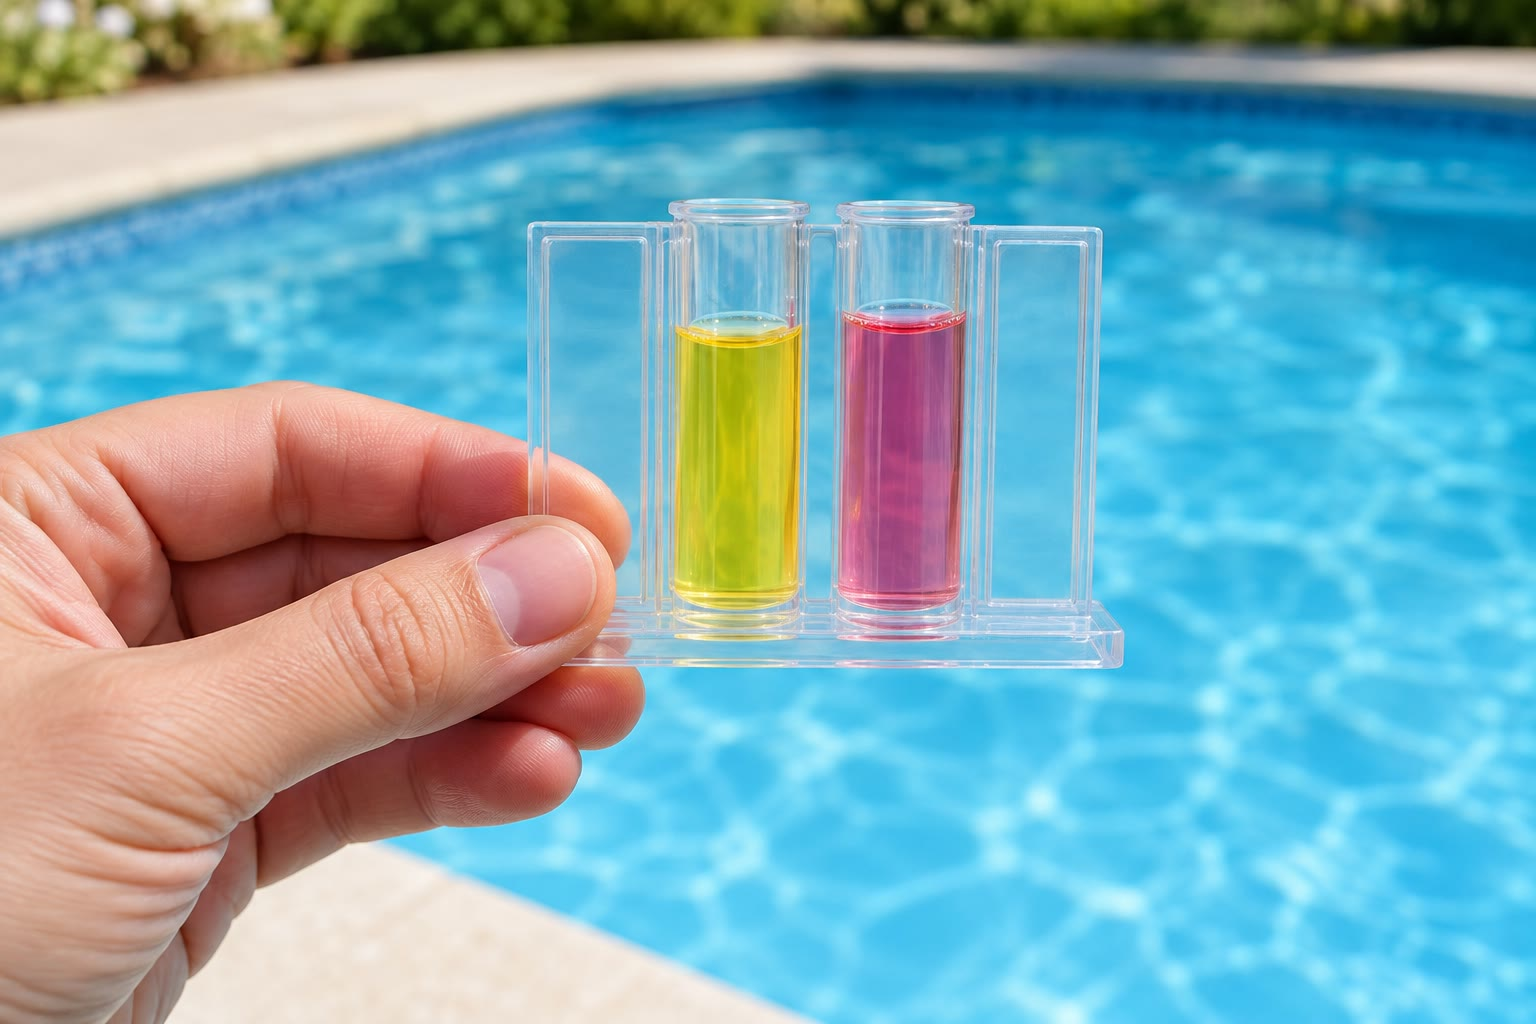
\includegraphics[width=0.45\linewidth]{images/book1/ai/g12-pool-test.jpg}

{\small 检测游泳池水的酸碱性：指示剂的颜色可给出
pH。}
\end{omfigure}

\section{练习}


\begin{exercise}[$\star$]\label{exo:g12:buffers-predominance:1}
共轭对 \ce{CH3COOH}/\ce{CH3COO-}（$pK_a = 4.76$）中，哪一种形式
在 pH 2、pH 4.76 和 pH 7 时占优势？
\end{exercise}

\begin{exercise}[$\star$]\label{exo:g12:buffers-predominance:2}
根据乙酸的分布图，读出
\ce{CH3COO-} 在 pH 4 和 pH 6 时的分布分数。
\end{exercise}

\begin{exercise}[$\star$]\label{exo:g12:buffers-predominance:3}
溴百里酚蓝在 pH 5、pH 7 和 pH 9 时分别显示什么颜色？
\end{exercise}

\begin{exercise}[$\star$]\label{exo:g12:buffers-predominance:4}
共轭对 \ce{NH4+}/\ce{NH3} 中，哪一种形式在
pH 7.4 的溶液中占优势？pH 11 时呢？
\end{exercise}

\begin{exercise}[$\star$]\label{exo:g12:buffers-predominance:5}
为什么指示剂的用量要很少？
\end{exercise}

\begin{exercise}[$\star\star$]\label{exo:g12:buffers-predominance:6}
计算 $[\ce{CH3COO-}]/[\ce{CH3COOH}]$ 在 pH 3.76、4.76 和
5.76 时的比值。
\end{exercise}

\begin{exercise}[$\star\star$]\label{exo:g12:buffers-predominance:7}
滴定终点为 pH 8.7。图中四种指示剂中，
你会选用哪一种？为什么不用甲基红？
\end{exercise}

\begin{exercise}[$\star\star$]\label{exo:g12:buffers-predominance:8}
一个缓冲溶液含 \qty{0.20}{mol/L} 的乙酸和
\qty{0.10}{mol/L} 的乙酸钠。求其 pH。
\end{exercise}

\begin{exercise}[$\star\star$]\label{exo:g12:buffers-predominance:9}
利用甘氨酸的分布图，给出 pH 1、6 和 12 时的
占优势形式及其所带电荷。
\end{exercise}

\begin{exercise}[$\star\star$]\label{exo:g12:buffers-predominance:10}
读取响应曲线：加入
\qty{1.0}{mL} 酸后，水的 pH 下降了多少？缓冲溶液的 pH 呢？
\end{exercise}

\begin{exercise}[$\star\star$]\label{exo:g12:buffers-predominance:11}
应从优势区域图中选择哪一对共轭对来配制
pH 为 9.5 的缓冲溶液？两种形式应按何比例混合？
\end{exercise}

\begin{exercise}[$\star\star\star$]\label{exo:g12:buffers-predominance:12}
图中的乙酸盐缓冲溶液（两种形式各 \qty{10}{mmol}）
加入盐酸。它的 pH 下降
一个单位之前能吸收多少盐酸？为什么较浓的缓冲溶液
被称为具有更大的缓冲容量？
\end{exercise}

\begin{exercise}[$\star\star\star$]\label{exo:g12:buffers-predominance:13}
需加入多大体积浓度为 \qty{0.10}{mol/L} 的乙酸钠溶液，
才能与 \qty{100}{mL} 浓度为 \qty{0.10}{mol/L} 的乙酸混合，得到
pH 为 5.0 的缓冲溶液？
\end{exercise}

\begin{exercise}[$\star\star\star$]\label{exo:g12:buffers-predominance:14}
百里酚蓝有两个变色范围。请解释原因，并给出其
在 pH 1、5 和 10 时的颜色。
\end{exercise}

\begin{exercise}[$\star\star\star$]\label{exo:g12:buffers-predominance:15}
将 pH 为 4.76 的缓冲溶液用蒸馏水稀释十倍，
按亨德森关系式，其新的 pH 为多少？若
将 pH 相同的强酸稀释十倍，会怎样？
\end{exercise}

\section{问题：血液的缓冲体系}

\begin{problem}[{周末问题——碳酸氢根与
二氧化碳之比为多少时，血液的 pH 保持在 7.4？}]
\label{pb:g12:buffers-predominance:1}
% ledger: pk:blood-bicarb, ph:blood, hco3:blood
动脉血的 pH 通常在 7.38 至 7.42 之间。其主要
缓冲体系是共轭对 \ce{CO2,H2O}/\ce{HCO3-}，生理学家对其采用
$\mathrm{pH} = 6.1 + \log\big([\ce{HCO3-}]/[\ce{CO2}]\big)$ 关系式。血液中正常的
碳酸氢根浓度为 22 至 \qty{28}{mmol/L}。

\medskip
\noindent\textbf{第一部分——共轭对。}
\begin{enumerate}
  \item 写出溶解的二氧化碳与水
        反应生成碳酸氢根离子的方程式。
  \item 哪种物质是酸，哪种是碱？
  \item 数值 6.1 与 $pK_a$ 表中的 6.37 不同。
        请给出一个原因（想一想人体的温度以及体系中存在的
        其他离子）。
  \item 在 \qty{24}{mmol/L} 的浓度下，\qty{5.0}{L} 血液
        中含碳酸氢根的物质的量为多少？
\end{enumerate}

\medskip
\noindent\textbf{第二部分——优势区域。}
\begin{enumerate}[resume]
  \item 画出 $pK = 6.1$ 的共轭对的优势区域图。
  \item 血液中哪种形式占优势？
  \item 血液呈弱酸性还是弱碱性？
\end{enumerate}

\medskip
\noindent\textbf{第三部分——比值。}
\begin{enumerate}[resume]
  \item 利用该关系式，计算 $[\ce{HCO3-}]/[\ce{CO2}]$
        在 pH 为 7.4 时的值。
  \item 已知 $[\ce{HCO3-}] = \qty{24}{mmol/L}$，计算 $[\ce{CO2}]$。
  \item 计算正常范围两端 7.38 与
        7.42 处的比值。
  \item 在 pH 为 7.4 时，该共轭对中以碳酸氢根形式
        存在的比例是多少？
  \item 若血液过于偏碱，pH 可能升至 7.6。
        此时的比值为多少？
\end{enumerate}

\medskip
\noindent\textbf{第四部分——平衡被打破时。}
\begin{enumerate}[resume]
  \item 剧烈运动时，酸进入血液。共轭对中哪种形式
        会消耗它们？写出反应方程式。
  \item 若 pH 降至 7.1，比值将变为多少？
  \item 保持碳酸氢根浓度不变，二氧化碳需增加
        多少？肺部如何作出应对？
  \item 为什么用弱酸及其共轭碱，而不是强酸，
        来稳定 pH？
  \item 若两种浓度均除以 2，pH 改变多少？
        为什么？
  \item 给出最终答案：pH 为 7.4 时，血液中碳酸氢根与
        二氧化碳的比值是多少？
\end{enumerate}
\end{problem}
